\documentclass[12pt,a4paper,titlepage]{article}
\usepackage{fullpage}
\usepackage{hyperref}
\usepackage[pdftex]{graphicx}
\bibliographystyle{plain}
\newcommand{\HRule}{\rule{\linewidth}{0.5mm}}
\usepackage{url}
\usepackage{amsmath}
\usepackage{enumitem}
\usepackage{float}
\usepackage{graphicx}
\usepackage{caption}
\usepackage{subcaption}
\usepackage{tabularx}
\usepackage[nottoc]{tocbibind}
\setlength{\parindent}{0.0in}
\setlength{\parskip}{0.1in}
\begin{document}

\begin{titlepage}
    \let\footnotesize\small
    \let\footnoterule\relax
    \let \footnote \thanks
    \setcounter{footnote}{0}
    \begin{center}
      \setlength{\parskip}{0pt}
       {\large School Of Electronics and Computer Science \par}
      {\large Faculty of Physical and Applied Sciences \par}
      {\large University of Southampton \par}
      \vspace{29mm}
      {\large Argyris Zardilis \par}	
	\vspace{4mm}
      \large \today
	\vspace{13mm}
        \center
        {\Large \bf Tool for parameter inference in dynamic biological systems \par}
        \vspace{60mm}
      {\large Project Supervisor: Dr. Srinandan Dasmahapatra \par }
      {\large Second Examiner: Dr. Markus Brede \par}
      \vspace{12mm}
        {\large A progress report submitted for the award of }\\
      {\large BSc Computer Science }
    \end{center}
    \vfil\null
  \end{titlepage}
\begin{abstract}
Recent advances in experimental technology have given us detailed and comprehensive information on networks of biological interactions governing various functions of living organisms. This had led to an increase in the use of theoretical mathematical models to describe dynamic biological systems which has in turn led to an increasing need for computational tools to assist in the process of constructing these models and estimating their parameters from available experimental data. Although there is a rich literature on parameter estimation using a number of different techniques, very few attempts have been made to systematically attack the parameter estimation problem for these kinds of systems. From those, almost all of them attempt a mere reproduction of experimental data, disregarding important properties of those systems like their qualitative features and the effect of global system dynamics. 

In this study a computational tool has been produced tackling the parameter estimation problem in dynamic biological systems using different techniques and its success has been tested with real world models. Further to that, an attempt has been made to uncover the link and interplay between the practical considerations of the parameter inference process and the more theoretical tools of sensitivity and bifurcation analysis and therefore consequently to systems dynamics which are captured and understood through these. 
\end{abstract}
\tableofcontents
\newpage
\section{Introduction}
Cells of living organisms contain thousands of networks of biochemical interactions that perform their functions. Despite being, at the molecular level, subject to thermal noise and the random tinkering of evolutionary events they are able to perform their functions almost always without error and with remarkable consistency. The apparent high complexity of such networks has been perhaps one of the reasons that the main bulk of biological research has been focused on understanding the details of individual components instead of a systems-level understanding of their interactions. So in a way Biology did not follow the route of other natural sciences, like Physics for example, to try and find simplifying and general principles and laws that govern the behaviour of the natural systems occurring in living organisms using the theoretical framework of Mathematics. It might be because the general consensus was that living organisms are so complex and their behaviour is so highly stochastic at the molecular level that one will not be able to find these laws and express them using a rigorous language like Mathematics as used for inanimate objects. 

However recent advances in experimental technology like microarray experiments which enabled us to get the expression levels of a big number of genes at different time points have given us for the first time such detailed and comprehensive information on cellular processes.  Although the structure of such interactions has been assembled from the effects of many random evolutionary events over time, with this new volume of information we  are able to find common reoccurring network structures which evolution keeps turning to because exactly they are the ones that survive with their robustness. This leads us to think that they are common design principles behind these common network motifs that drive them so the goal of finding generalising and simplifying principles and gain systems level understanding through a theoretical framework inside the apparent complexity is revisited recently shifting some of the attention of biological research from experimentation to more theoretical work\cite{alon2007introduction}. Commonly occurring motifs (network structures) include switches, buzzers, blinkers\cite{tyson2003sniffers}, the inspiration for the decomposition and naming also coming from their resemblance to electronic-like components.

These common network motifs can then be assembled and be parts of larger networks of interactions that perform more complicated functions.  Such networks that their network structure is though to be well understood and have been the subject of much study both experimentally but even more theoretically include circadian oscillators and metabolic pathways\cite{bass2010circadian, sahar2012regulation, mirsky2009model}. As their name suggests one of the main properties of such networks of interactions is their structure, what are the interacting components and which one acts on what. The traditional way to capture this structure is with schematic means with the aid of a diagram an example of which can be seen in Figure \ref{fig:diagram_example}. Components of the networks are gene mRNA products and proteins which can either serve a biochemical function or act as transcription factors for genes. Transcription factors can act on genes to either activate:increase the rate of production or repress:decrease the rate of production of one or more genes. The gene products themselves though control the production of other proteins which can act as transcription factors(activators or repressors) to other genes or even themselves thus creating networks of interactions of varying complexity. The components of the network are the nodes of the diagram with their differences highlighted with the use of different shapes or colours while the interactions(regulations) are the edges differentiated by their ends; for example the flat end signifies repression while the arrow signifies activation. Several attempts to standardise these diagrams in the example of circuit diagrams in electronics (Molecular Interaction Maps\cite{kohn2006molecular}) have not been widely adopted so they still vary considerably across publications.
\begin{figure}
\centering
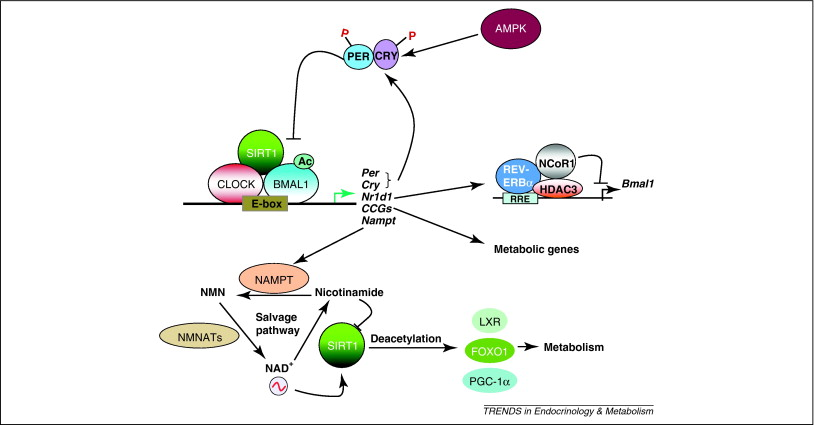
\includegraphics[width=0.9\linewidth]{clock_metabolism}
\caption{Networks of interactions between circadian clock and metabolic pathways\cite{sahar2012regulation}}

\label{fig:diagram_example}
\end{figure}

The network structure, though important, is only one of the properties that help us get insight into the workings of these systems. Another essential property which becomes even more apparent as the diagrams and networks grow in size is the systems dynamics. The diagrammatic way of describing the systems is very poor in that sense as it does not capture the dynamic properties that these systems exhibit\cite{kitano2002computational}. The natural way to capture the dynamic behaviour of systems that is being used throughout science is with differential equations. That way we can use a more theoretical and well researched framework of Mathematics and of dynamical systems in particular  to talk about these systems and borrow tools from it that aid the analysis process and give us greater insight to eventually build a systems-level understanding of complex biological systems. %write something about the further goal, synthetic biology durg design etc.
The we can ask more complicated and interesting questions like: what are the control mechanisms that drive these systems? how does one part affect others? Which parts provide the stability and robustness to the system? How will the system behave in the future with the same or varying conditions? The diagrams which offer the static structure provide very little knowledge and surely cannot answer these questions.

Systems can be thought of as stochastic processes as they are subject to molecular noise and various fluctuations in their interactions. Therefore they can be expressed as stochastic differential equations or their evolution can be simulated with the Gillespie algorithm\cite{gillespie1977exact} or one of its more recent variants\cite{gillespie2001approximate, gibson2000efficient}. However the effects of these fluctuations are only considerable when the number of molecules of the reactants is very small so more often the average case is considered and the systems are expressed as deterministic Ordinary Differential Equations(ODEs) like so: 
\begin{equation*}
\mathbf{\dot x} = \mathbf{F}(\mathbf{x}, t, \mathbf{\theta})
\end{equation*}
 These describe the evolution in the concentrations of components of the systems(variables) over time and are parameterised by $\mathbf{\theta}$ which mainly describes the kinetic rates of the reactions/regulation or other constants like initial concentrations. So the evolution of the concentration of component $x1$ might be described by $f(\mathbf{x}, t, \theta)$ which tells us how the concentration is altered through the effects of other variables(components) or itself over time. These equations are translations of the diagrams and the duality of the representation can be seen through an example. Let's consider the a simple synthetic network motif seen in Figure\ref{fig:simple_motif}. 
\begin{figure}
\centering
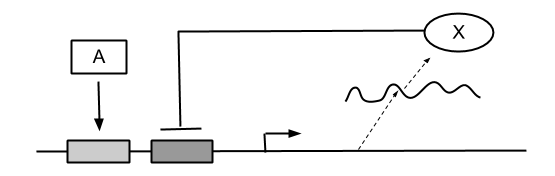
\includegraphics[width=0.5\linewidth]{neg_autoregulation}
\caption{Negative autoregulation network motif: Gene X and its protein product are regulated by A. Protein product X also represses its own production\cite{alon2007introduction}(chapter 1)}
\label{fig:simple_motif}
\end{figure}
This is a common negative autoregulation motif which occurs in 40\% of known transcription factors in E.Coli\cite{rosenfeld2002negative}. In this network gene X(and its protein product) is regulated by A. The protein X acts as a transcription factor for its own gene repressing its own production. We are concerned with the concentration of protein product X so that is one of our variables. Now we need to express the change in its concentration as an equation. The production of protein X is balanced by the dilution due to the growing area of the cell and the degradation due to its natural destruction. Therefore the change in the concentration can be expressed as the difference between the two processes(production and dilution/degradation).  The regulation of X by A(transcription and translation) is orders of magnitude faster than the change in the concentration of X so we can assume the production rate due to A's regulation is constant at a rate $\beta$. However the production rate is also affected negatively by X itself so it should be a decreasing function of X with $\beta$ as its maximum value when $X=0$. One such function that is found to agree with observation is the Hill function: $ f(X) = \frac{\beta}{1 + \left(\frac{X}{K}\right)^n}$. The dilution/degradation process at a rate $\alpha$ is proportional to its concentration so the resulting differential equation for the concentration of X is:
\begin{equation}
\frac{dX(t)}{dt} = \frac{\beta}{1 + \left(\frac{X}{K}\right)^n} - \alpha X
\label{eq:neg_autoregulation}
\end{equation}
The Hill equation for the repressor can be derived from simple chemical kinetic laws like the law of mass-action\cite{} or Michaelis-Menten kinetics\cite{}(see Appendix A in \cite{alon2007introduction} for a detailed derivation and explanation). Starting from these simple laws one can describe as equations all reactions and therefore all systems. The intuition and background knowledge of the modeler though is needed for simplifying the models, for example as we have done for the transcription factor A where we treated it as constant due the differences in timescales between the processes(Quasi-steady-state approximation). 

For this simple model, one could easily understand the dynamics of it just by looking at it. However for most systems this is not very easy and most of these systems cannot be solved analytically. This is where the knowledge from the field of dynamical systems comes in. One of the main observations and driving force in field of dynamical systems is: we cannot solve these systems analytically so how can we understand their dynamic behaviour from the differential equations themselves. Of course now we can solve these systems numerically and get  good idea of how these systems evolve over time. To solve numerically though we need values for the parameter quantities like $\beta, K, n, \alpha$ in Eq\ref{eq:neg_autoregulation}. These parameters in these models have a physical interpretation: production/degradation rates, binding affinities, transport rates, etc. This generally poses an issue because quantitative data on these parameters are rarely available because they are difficult to measure experimentally. 

The problem therefore is to estimate those parameter values from experimental measurements of the concentrations of the network components over a time period, data which might be scarce or incomplete. This problem sometimes called the inverse problem can be seen as going from the real world observables to the mathematical models that represent those observables. Doing that for parametric models is equivalent to finding the parameters. This inverse problem is a common theme in Machine Learning so there is a large toolbox of available techniques to tackle the problem. However these classical methods are not always suited to such complex systems and might fail. Moreover there are more factors that come into play as far as biological systems are concerned which are not captured by these techniques. The increase in the available computational power has made possible the introduction of new techniques which are based on simulation which have been shown to be more suited to the task. However there have been very few attempts to produce computational tools that aid in the modeling process and attack this problem in this domain despite its importance(see \ref{sec:background} for a more detailed treaty on parameter estimation methods used in this domain and relevant tools). It is with this inference problem and these new techniques that this study is concerned with.  The first part of this project has been to use these new techniques to produce a computational tool that automatically and systematically attacks the parameter estimation problem. Discussion and results are covered in chapter 1 of this study. 

\begin{figure}
\centering
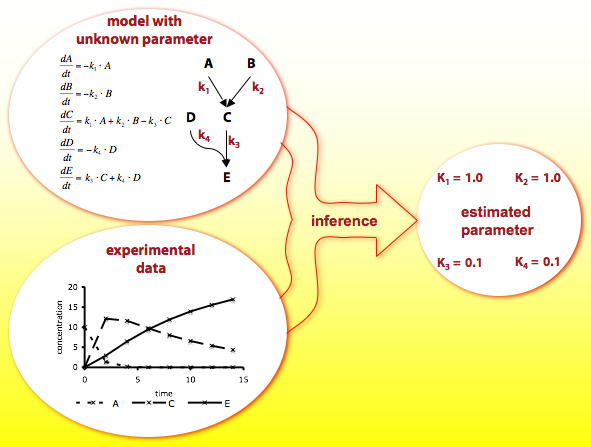
\includegraphics[width=0.5\linewidth]{inference}
\caption{Parameter inference methods combine experimental data with the knowledge about the underlying structure of a dynamical system to be investigated. Unknown model parameter (here k1, k2, k3 and k4) can be estimated.}
\label{fig:inference}
\end{figure}

Work on the first task of this project has led to some observations that potentially link the parameter estimation procedure with some more theoretical tools and aspects of the systems in question.  
As has been previously discussed systems dynamics play an important role in our understanding of complex biological systems. The language of choice for their description(differential equations) enables us to use some of the tools developed in the field of dynamical systems to investigate the dynamics. Simple models like the one for the negative autoregulation network motif described previously are easy to understand intuitively but as the models grow intuition alone cannot help. Sensitivity analysis on these models tells us how much the observable behaviour of the system depends on specific parameters of the model. The second part of this study is firstly concerned with the connection between the practical considerations of parameter estimation and the more theoretical tool of sensitivity analysis. Is there a connection between the estimate for a parameter and the model's sensitivity to it? Bifurcation is a change in a system's dynamics as one of its parameters passes through a bifurcation point. In parameter estimation the effects of global dynamics are hardly ever considered despite the fact that their importance in understanding biological systems has been demonstrated\cite{}. Do these global dynamics affect the parameter estimation procedure? This is also something that we try to address in the second part of this study.


\section{Background Research}
\label{sec:background}
The parameter estimation problem as posed in the previous section is the inverse problem of going from world observables to models that represent those observables. To formalise this problem, we have a proposed model for our system which describes the evolution of all variables(components) $\mathbf{x} = \{x_1, x_2, \dots, x_n\}$ like so:
\begin{equation}
\label{eq:system}
\begin{array}{lcl}
\dot x_1 & = & f(\mathbf{x}, t, \theta) \\
\dot x_2& = & f(\mathbf{x}, t, \theta) \\
\vdots \\
\dot x_n & = & f(\mathbf{x}, t, \theta) \\
\end{array}
\end{equation}
We also have the observations of the world in the form of experimental data at $N$ different time points like so $\mathbf{Y_d} = \{\mathbf{y}_{t_{1}},  \mathbf{y}_{t_{2}}, \dots, \mathbf{y}_{t_{N}}\}$ where the obseration at time point $t_{k}$ tells the state of the system(concentration of $n$ variables) at that point so 
$\mathbf{y}_{t_{k}} =\{ x_{1}^{t_{k}},  x_{2}^{t_{k}}, \dots,  x_{n}^{t_{k}} \}$. The problem then become to find the parameter vector $\theta^*$ from the set of all the possible parameter vectors $\mathbf{\Theta}$ so that the model $\mathbf{\dot x} = \mathbf{F}(\mathbf{x}, t, \mathbf{\theta^*})$  \ref{eq:system} fits the experimental data best. The fitness of a particular parameter vector $\theta_{s}$ can be assessed with a distance metric between the experimental data $\mathbf{Y}_{d}$ and a simulated solution $\mathbf{Y}_{s}$ for proposed parameter $\theta_{s}$. Then the problem becomes the minimisation of this distance metric. Then this is a common optimisation problem formulation: 
\begin{equation*}
\theta^* = \underset{\theta}{\arg\min}(d(\mathbf{Y_{d}},\mathbf{Y}_{s})) 
\end{equation*}
where $d$ is some distance metric or the cost function in optimisation language. Naturally much attention has been given on parameter estimation for deterministic systems with local and global optimisation methods\cite{Moles2003param}.

\section{Parameter Estimation}
\subsection{Methods}

\subsection{Results}

\section{Discussion and Future Work}

\newpage
\bibliography{report}
\appendix
\section{Time Management}
\section{Critical Evaluation}
\end{document}